\newcommand{\SB}{ShrinkBench}
\newcommand{\NEXP}{800} % but that's counting the activation methods


\vspace{1mm}

% \subsection{}

% Because many of the above suggestions require extra work, we have created an open-source library---ShrinkBench---to facilitate adherence to each of them.

% ------------------------------------------------
\subsection{Overview of ShrinkBench}
% ------------------------------------------------

To make it as easy as possible for researchers to put our suggestions into practice, we have created an open-source library for pruning called ShrinkBench. % \footnote{Source code is available at \url{https://github.com/jjgo/shrinkbench}}.
ShrinkBench provides standardized and extensible functionality for training, pruning, fine-tuning, computing metrics, and plotting, all using a standardized set of pretrained models and datasets.

ShrinkBench is based on PyTorch \cite{pytorch} and is designed to allow easy evaluation of methods with arbitrary scoring functions, allocation of pruning across layers, and sparsity structures. In particular, given a callback defining how to compute masks for a model's parameter tensors at a given iteration, ShrinkBench will automatically apply the pruning, update the network according to a standard training or fine-tuning setup, and compute metrics across many models, datasets, random seeds, and levels of pruning.
We defer discussion of ShrinkBench's implementation and API to the project's documentation.

% ------------------------------------------------
\subsection{Baselines}
% ------------------------------------------------

We used ShrinkBench to implement several existing pruning heuristics, both as examples of how to use our library and as baselines that new methods can compare to:
\begin{itemize}[leftmargin=4mm]
    \itemsep-1pt
    % \itemsep2pt
    \vspace{-2mm}
    \item \textbf{Global Magnitude Pruning} - prunes the weights with the lowest absolute value anywhere in the network.
    \item \textbf{Layerwise Magnitude Pruning} - for each layer, prunes the weights with the lowest absolute value.
    \item \textbf{Global Gradient Magnitude Pruning} - prunes the weights with the lowest absolute value of (weight $\times$ gradient), evaluated on a batch of inputs.
    \item \textbf{Layerwise Gradient Magnitude Pruning} - for each layer, prunes the weights the lowest absolute value of (weight $\times$ gradient), evaluated on a batch of inputs.
    \item \textbf{Random Pruning} - prunes each weight independently with probability equal to the fraction of the network to be pruned.
\end{itemize}
% \vspace{-1mm}
\vspace{-2mm}

Magnitude-based approaches are common baselines in the literature and have been shown to be competitive with more complex methods \cite{learning-both, han-prune-quant-huff, google-state-of-sparsity, lottery-ticket-followup}. Gradient-based methods are less common, but are simple to implement and have recently gained popularity \cite{snip, snip-followup, nisp}. Random pruning is a common straw man that can serve as a useful debugging tool. Note that these baselines are not reproductions of any of these methods, but merely inspired by their pruning heuristics.

% \vps
\subsection{Avoiding Pruning Pitfalls with Shrinkbench}

Using the described baselines, we pruned over \NEXP{} networks with varying datasets, networks, compression ratios, initial weights and random seeds.
%
In doing so, we identified various pitfalls associated with experimental practices that are currently common in the literature but are avoided by using ShrinkBench.
% We found ShrinkBench's standardized and thorough evaluation to be helpful when comparing pruning methods.

We highlight several noteworthy results below. For additional experimental results and details, see Appendix~\ref{apx:res}.  One standard deviation bars across three runs are shown for all CIFAR-10 results.

\vspace{-2mm}
\paragraph{Metrics are not Interchangeable.}
As discussed previously, it is common practice to report either reduction in the number of parameters or in the number of FLOPs. If these metrics are extremely correlated, reporting only one is sufficient to characterize the efficacy of a pruning method. We found after computing these metrics for the same model under many different settings that reporting one metric is not sufficient. While these metrics are correlated, the correlation is different for each pruning method. Thus, the relative performance of different methods can vary significantly under different metrics (Figure~\ref{fig:ImageNet_flops}).
\begin{figure}[h]
\begin{center}
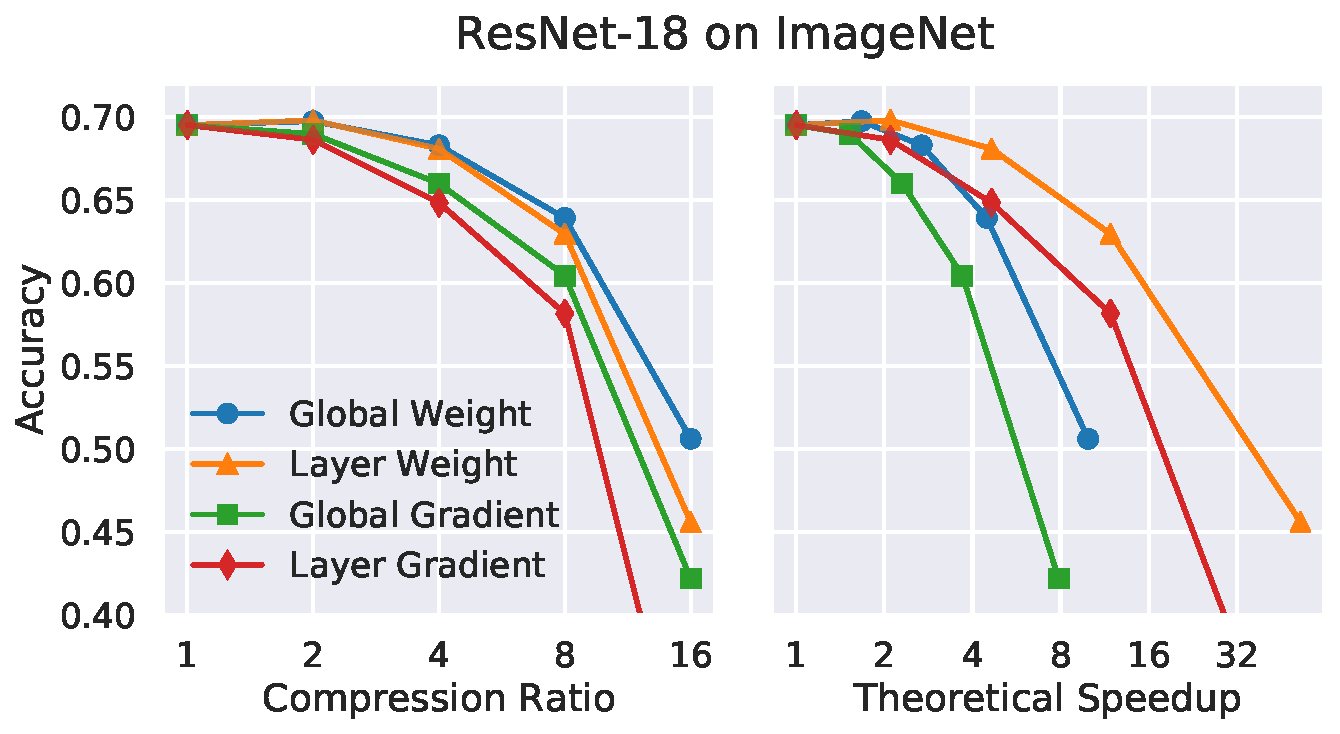
\includegraphics[width=\linewidth]{shrinkbench/ImageNet_flops}
% \vspace{-3mm}
\caption{Top 1 Accuracy for ResNet-18 on ImageNet for several compression ratios and their corresponding theoretical speedups.
%
Global methods give higher accuracy than Layerwise ones for a fixed model size, but the reverse is true for a fixed theoretical speedup.
}
\label{fig:ImageNet_flops}
\end{center}
\vspace*{-3mm}
\end{figure}

\vspace{-3mm}
\paragraph{Results Vary Across Models, Datasets, and Pruning Amounts}

Many methods report results on only a small number of datasets, models, amounts of pruning, and random seeds. If the relative performance of different methods tends to be constant across all of these variables, this may not be problematic. However, our results suggest that this performance is not constant.

Figure \ref{fig:sb_CIFAR10} shows the accuracy for various compression ratios for CIFAR-VGG \cite{vggCifarTorch} and ResNet-56 on CIFAR-10.
In general, Global methods are more accurate than Layerwise methods and Magnitude-based methods are more accurate than Gradient-based methods, with random performing worst of all.
However, if one were to look only at CIFAR-VGG for compression ratios smaller than 10, one could conclude that Global Gradient outperforms all other methods.
Similarly, while Global Gradient consistently outperforms Layerwise Magnitude on CIFAR-VGG, the opposite holds on ResNet-56 (i.e., the orange and green lines switch places).
% This is the opposite of the conclusion one would reach using ResNet-56, where that method is always outperformed by Global and Layerwise Magnitude Pruning.
%
% This shows the need to evaluate on a pruning method on various model and dataset combinations to ensure it is not architecture dependent.
%
% Similarly, this shows the need to report metrics for several compression rations to characterize the trade-off curve as pruning increases.
%

Moreover, we found that for some settings close to the drop-off point (such as Global Gradient, compression 16), different random seeds yielded significantly different results (0.88 vs 0.61 accuracy) due to the randomness in minibatch selection. This is illustrated by the large vertical error bar in the left subplot.

\begin{figure}[h]
\begin{center}
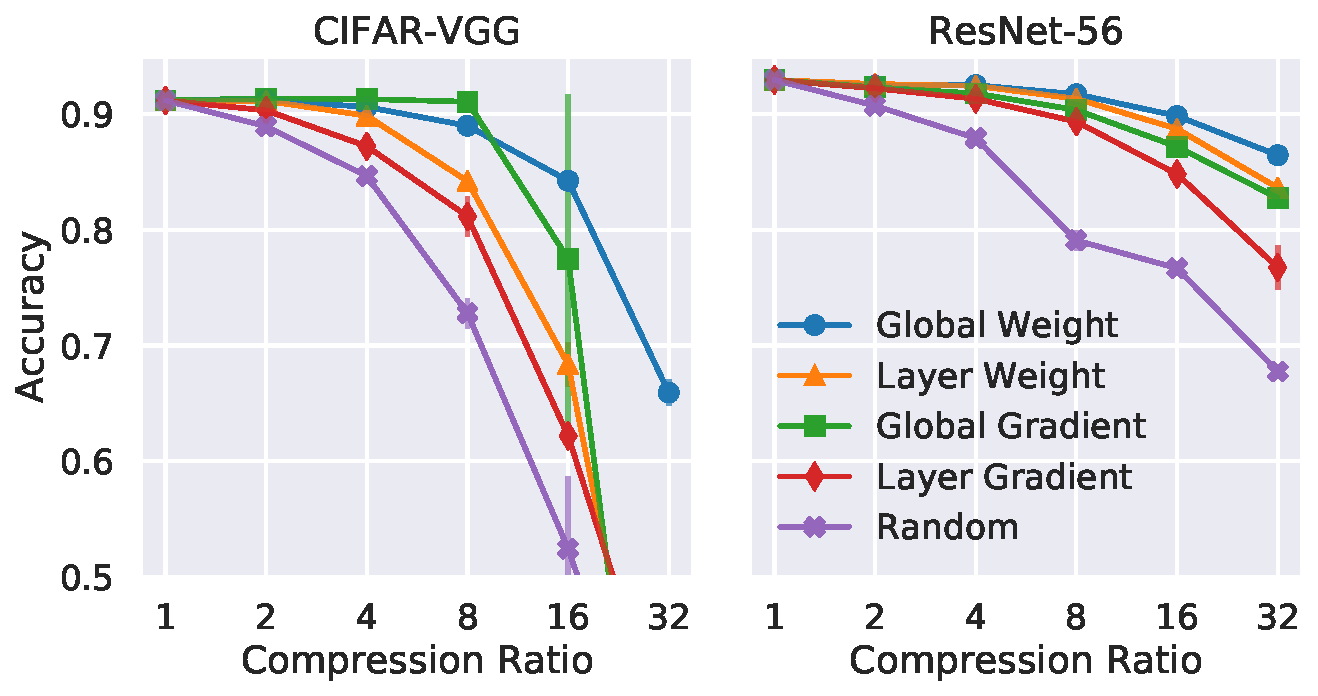
\includegraphics[width=\linewidth]{shrinkbench/CIFAR10_models}
% \vspace{-3mm}
\caption{Top 1 Accuracy on CIFAR-10 for several compression ratios.
%
 Global Gradient performs better than Global Magnitude for CIFAR-VGG on low compression ratios, but worse otherwise.
 Global Gradient is consistently better than Layerwise Magnitude on CIFAR-VGG, but consistently worse on ResNet-56.
 %
 % One standard deviation bars across three runs are included for all compression ratios greater than one.
}
\label{fig:sb_CIFAR10}
\end{center}
\end{figure}


% In absolute accuracy, Global strictly outperforms Layerwise Magnitude for both sets of pretrained weights.
% However, if we compare Layerwise Magnitude with pretrained weights A and Global with pretrained weights B, the previous conclusion could not be drawn.
%
% This is due to the fact that Layerwise with pretrained weights B has a smaller change in accuracy than Global with pretrained weights A for high compression ratios.
%
% This shows the need to use the same set of pretrained weights when comparing pruning methods since it can be a confounding factor.

\vspace{-4mm}
\paragraph{Using the Same Initial Model is Essential.}

As mentioned in Section~\ref{sec:confounding}, many methods are evaluated using different initial models with the same architecture. To assess whether beginning with a different model can skew the results, we created two different models and evaluated Global vs Layerwise Magnitude pruning on each with all other variables held constant.

To obtain the models, we trained two ResNet-56 networks using Adam until convergence with $\eta=10^{-3}$ and $\eta=10^{-4}$.
We'll refer to these pretrained weights as Weights A and Weights B, respectively.
% Figure \ref{fig:sb_resnet56_confounding} shows pruning results for these two sets of initial weights using each pruning method at several compression ratios.
%
As shown on the left side of Figure~\ref{fig:sb_resnet56_confounding}, the different methods appear better on different models. With Weights A, the methods yield similar absolute accuracies. With Weights B, however, the Global method is more accurate at higher compression ratios.

% We also see that the common practice of examining changes in accuracy is insufficient to correct for initial model as a confounder. In absolute accuracy, Global strictly outperforms Layerwise Magnitude Pruning for both sets of pretrained weights.
%
% However, if we compare Layerwise pruning with pretrained weights A and Global with pretrained weights B, the previous conclusion could not be drawn.
%
% This is due to the fact that Layerwise with pretrained weights B has a smaller change in accuracy than Global with pretrained weights A for high compression ratios.
%
% This shows the need to use the same set of pretrained weights when comparing pruning methods since it can be a confounding factor.

\begin{figure}[t]
\begin{center}
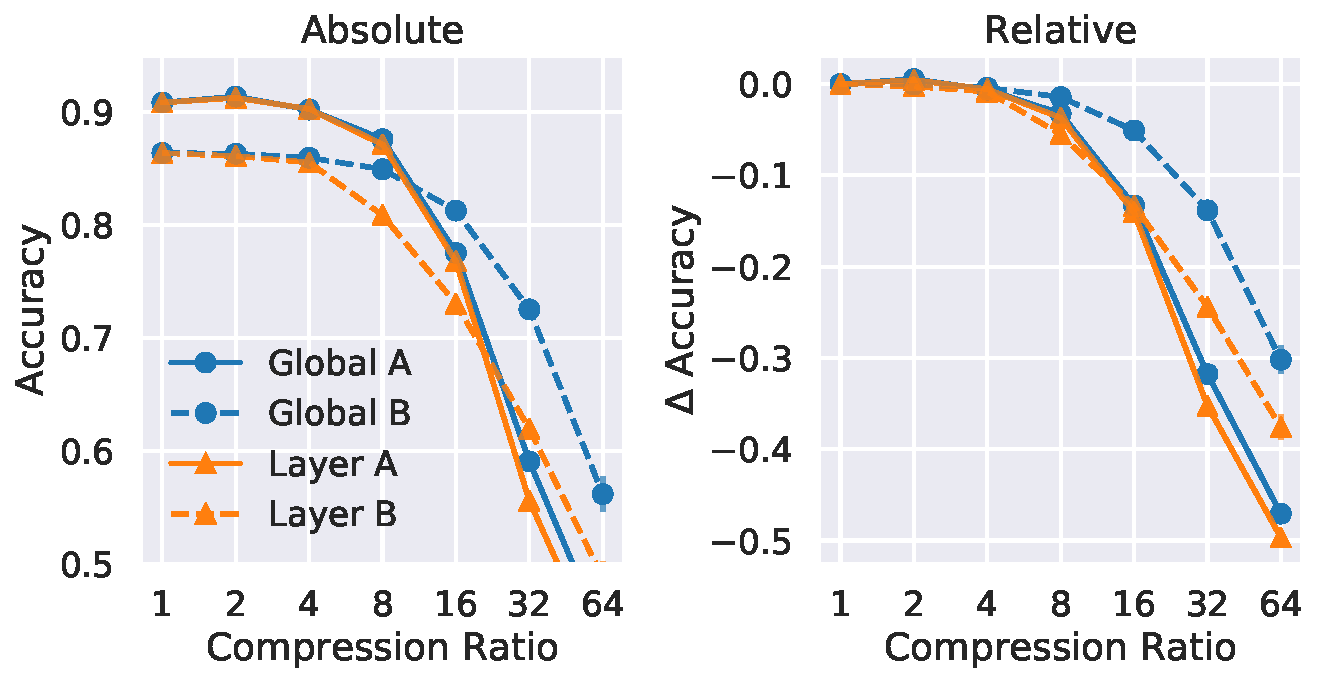
\includegraphics[width=\linewidth]{shrinkbench/confounding_resnet56}
% \vspace{-3mm}
\caption{Global and Layerwise Magnitude Pruning on two different ResNet-56 models.
%
% The starting models were obtained by training with Adam for 150 epochs with $\eta=10^{-3}$ (A) and $\eta=10^{-4}$ (B) respectively.
%
% One standard deviation bars across three runs are included for all compression ratios greater than one.
Even with all other variables held constant, different initial models yield different tradeoff curves. This may cause one method to erroneously appear better than another. Controlling for initial accuracy does not fix this. % problem.
% instead of raw accuracies, does not fix this problem.
}
\label{fig:sb_resnet56_confounding}
\end{center}
\end{figure}
We also found that the common practice of examining changes in accuracy is insufficient to correct for initial model as a confounder. Even when reporting changes, one pruning method can artificially appear better than another by virtue of beginning with a different model. We see this on the right side of Figure~\ref{fig:sb_resnet56_confounding}, where Layerwise Magnitude with Weights B appears to outperform Global Magnitude with Weights A, even though the former never outperforms the latter when initial model is held constant.

% Following \cite{google-state-of-sparsity}, we refrain from pruning

% \subsection{Design Goals}



